\documentclass[letterpaper]{article}
\usepackage[margin=1in]{geometry}
\usepackage[utf8]{inputenc}
\usepackage{textcomp}
\usepackage{amssymb}
\usepackage{natbib}
\usepackage{graphicx}
\usepackage{gensymb}
\usepackage{amsthm, amsmath, mathtools}
\usepackage[dvipsnames]{xcolor}
\usepackage{enumerate}
\usepackage{mdframed}
\usepackage[most]{tcolorbox}
\usepackage{csquotes}
% https://tex.stackexchange.com/questions/13506/how-to-continue-the-framed-text-box-on-multiple-pages

\tcbuselibrary{theorems}

\newcommand{\R}{\mathbb{R}}
\newcommand{\Z}{\mathbb{Z}}
\newcommand{\N}{\mathbb{N}}
\newcommand{\Q}{\mathbb{Q}}
\newcommand{\C}{\mathbb{C}}
\newcommand{\code}[1]{\texttt{#1}}
\newcommand{\mdiamond}{$\diamondsuit$}
\newcommand{\PowerSet}{\mathcal{P}}
\newcommand{\Mod}[1]{\ (\mathrm{mod}\ #1)}
\DeclareMathOperator{\lcm}{lcm}

%\newtheorem*{theorem}{Theorem}
%\newtheorem*{definition}{Definition}
%\newtheorem*{corollary}{Corollary}
%\newtheorem*{lemma}{Lemma}
\newtheorem*{proposition}{Proposition}


\newtcbtheorem[number within=section]{theorem}{Theorem}
{colback=green!5,colframe=green!35!black,fonttitle=\bfseries}{th}

\newtcbtheorem[number within=section]{definition}{Definition}
{colback=blue!5,colframe=blue!35!black,fonttitle=\bfseries}{def}

\newtcbtheorem[number within=section]{corollary}{Corollary}
{colback=yellow!5,colframe=yellow!35!black,fonttitle=\bfseries}{cor}

\newtcbtheorem[number within=section]{lemma}{Lemma}
{colback=red!5,colframe=red!35!black,fonttitle=\bfseries}{lem}

\newtcbtheorem[number within=section]{example}{Example}
{colback=white!5,colframe=white!35!black,fonttitle=\bfseries}{def}

\newtcbtheorem[number within=section]{note}{Important Note}{
        enhanced,
        sharp corners,
        attach boxed title to top left={
            xshift=-1mm,
            yshift=-5mm,
            yshifttext=-1mm
        },
        top=1.5em,
        colback=white,
        colframe=black,
        fonttitle=\bfseries,
        boxed title style={
            sharp corners,
            size=small,
            colback=red!75!black,
            colframe=red!75!black,
        } 
    }{impnote}
\usepackage[utf8]{inputenc}
\usepackage[english]{babel}
\usepackage{fancyhdr}
\usepackage[hidelinks]{hyperref}

\pagestyle{fancy}
\fancyhf{}
\rhead{CSE 101}
\chead{Wednesday, January 26, 2022}
\lhead{Lecture 9}
\rfoot{\thepage}

\setlength{\parindent}{0pt}

\begin{document}

\section{Fundamental Shortest Paths Formula}
For any vertex $w$ that isn't the source $s$, $w \neq s$,
\[\text{dist}(w) = \min_{(v, w) \in E} \text{dist}(v) + \ell(v, w)\]
This says that the distance of $w$ is equal to the minimum over all edges $v$ to $w$ in $E$ of the distance to $v$ plus the length of the edge from $v$ to $w$. 
\begin{center}
    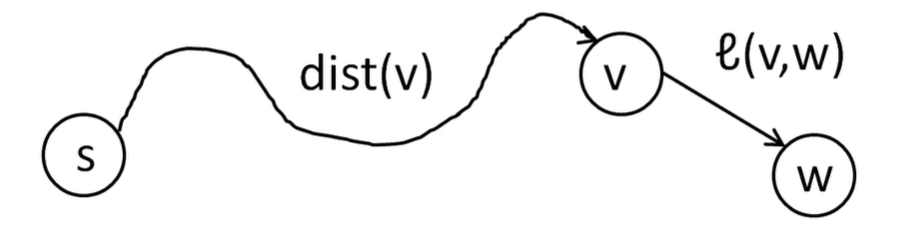
\includegraphics[scale=0.4]{../assets/fun_sho_path.png}
\end{center}
Looking at the visualization above, we're saying that the path from $s$ to $v$ has length $\text{dist}(v)$; this is the shortest path from $s$ to $v$.

\bigskip 

We can use a system of equations to solve for the distances from $s$ to ever other vertex in the graph. When $\ell \geq 0$, Dijsktra gives an order to solve in. But, with negative edge weights, this order is no longer clear. 

\subsection{Algorithm Idea}
Instead of finding the shortest paths, which may not exist due to a negative edge cycle, we instead find the shortest paths of length at most $k$ edges. So, for $w \neq s$, we have: 
\[\text{dist}_{k}(w) = \min_{(v, w) \in E} \text{dist}_{k - 1}(v) + \ell(v, w)\]
\begin{center}
    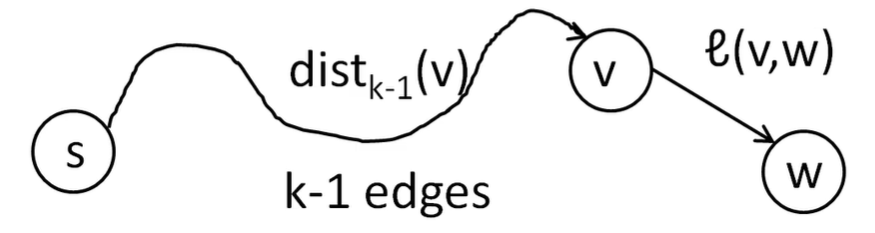
\includegraphics[scale=0.4]{../assets/fun_sho_path_2.png}
\end{center}
If we look at a path from $s$ to $w$ with at most $k$ edges, this is a path from $s$ to $v$ that uses at most $k - 1$ edges for some $v$ plus a single edge from $v$ to $w$. The best length this path could have is $\text{dist}_{k - 1}(v) + \ell(v, w)$, where our $\text{dist}_{k - 1}(v)$ is minimized. 

\subsection{Bellman-Ford Algorithm}
This formula gives rise to the \emph{Bellman-Ford} algorithm. 
\begin{verbatim}
    Bellman-Ford(G, s, l)
        dist_{0}(v) = infinity for all v 
        dist_{0}(s) = 0
        For k = 1 to n
            For w in V
                dist_{k}(w) = min(dist_{k}(w), dist_{k - 1}(v) + l(v, w))
            dist_{k}(s) = min(dist_{k}(s), 0)
\end{verbatim}
We note that each iteration of the outer-loop is $\BigO(|E|)$ time. However, what value of $k$ do we use? 

\subsubsection{Example: Applying the Bellman-Ford Algorithm}
Find the shortest path from $s$ to every other vertex in the graph shown below. For convenience, let the top-left vertex be denoted $A$, the top-right vertex be $B$, and the bottom-right vertex be $C$. 
\begin{center}
    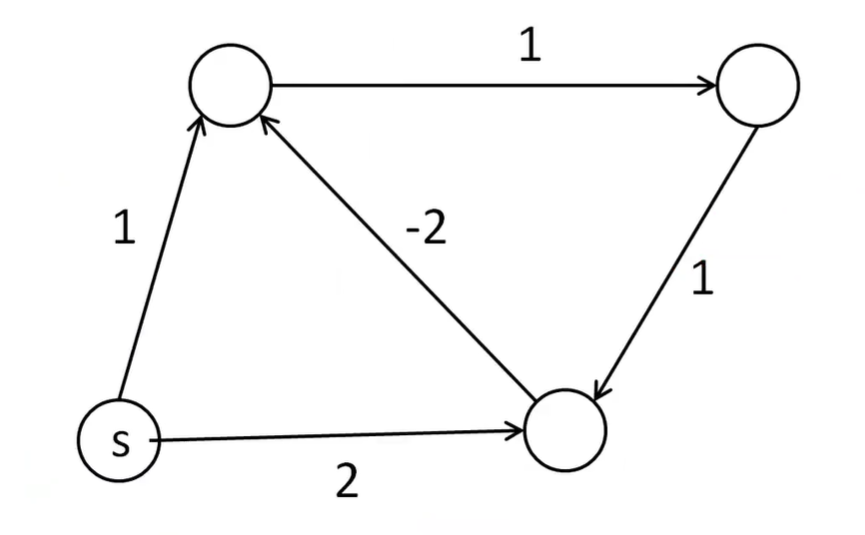
\includegraphics[scale=0.4]{../assets/shortest_path_problem.png}
\end{center}

\begin{mdframed}[]
    \begin{itemize}
        \item First, when $k = 0$, $s = 0$ and everything else is assigned $\infty$; you can't get to anywhere else with no edges. Therefore, the distances are: 
        \begin{center}
            \begin{tabular}{c|c c c c}
                $k$ & $s$   & $A$       & $B$       & $C$ \\ 
                \hline 
                0   & 0     & $\infty$  & $\infty$  & $\infty$
            \end{tabular}
        \end{center}

        \item When $k = 1$, we consider all vertices that we can reach with one edge. So, you still can't reach vertex $B$ since it needs at least two edges. But, we can get from $s$ to $A$ with path length 1, and we can get from $s$ to $C$ with path length 2. So: 
        \begin{center}
            \begin{tabular}{c|c c c c}
                $k$ & $s$   & $A$       & $B$       & $C$ \\ 
                \hline 
                0   & 0     & $\infty$  & $\infty$  & $\infty$ \\ 
                1   & 0     & 1         & $\infty$  & 2
            \end{tabular}
        \end{center}
        In other words, these are the shortest distances we can get from a path of length one to each of our vertices. 

        \item When $k = 2$, we consider all vertices that we can reach with two edges. First, we can reach vertex $B$ with just two edges (from $s$ to $A$ and from $A$ to $B$). $A$ has distance 1 so $B$ must have distance 2. We can't do any better with $s$ or $C$, but note that we can actually improve $A$ (if we go from $s$ to $C$ and from $C$ to $A$) by getting it down to distance 0. Therefore: 
        \begin{center}
            \begin{tabular}{c|c c c c}
                $k$ & $s$   & $A$       & $B$       & $C$ \\ 
                \hline 
                0   & 0     & $\infty$  & $\infty$  & $\infty$ \\ 
                1   & 0     & 1         & $\infty$  & 2 \\ 
                2   & 0     & 0         & 2         & 2
            \end{tabular}
        \end{center}

        \item When $k = 3$, we consider all vertices that we can reach with three edges. So, we can again reach every vertex. In particular, note we can update vertex $B$'s distance. This is because if $A$ is 0, then there is a path from $A$ to $B$ that has length 1 ($s \to C \to A \to B$). So: 
        \begin{center}
            \begin{tabular}{c|c c c c}
                $k$ & $s$   & $A$       & $B$       & $C$ \\ 
                \hline 
                0   & 0     & $\infty$  & $\infty$  & $\infty$ \\ 
                1   & 0     & 1         & $\infty$  & 2 \\ 
                2   & 0     & 0         & 2         & 2 \\ 
                3   & 0     & 0         & 1         & 2
            \end{tabular}
        \end{center}

        \item Past $k = 3$, we notice that the distances no longer change. In other words, the process has stabilized. 
    \end{itemize}
\end{mdframed}

\subsection{Analysis}
\begin{proposition}
    If $n \geq |V| - 1$ and if $G$ has no negative weight cycles, then for all $v$,
    \[\text{dist}(v) = \text{dist}_{n}(v)\]
\end{proposition}
This says that if we run the Bellman-Ford algorithm, there is a limit. Assuming there are no negative weight cycles\footnote{If there is a negative weight cycle, there is probably no shortest path.}, we only need to run the algorithm for $|V| - 1$ rounds for a final runtime of $\BigO(|V||E|)$.

\begin{mdframed}[]
    \begin{proof}
        We need to show that the shortest path has fewer than $|V|$ edges. Suppose that there is a path that has at least $|V|$ edges, then by the pigeonhole principle, it must contain the same vertex twice. This means that there is a loop. If we remove the loop (which we assume has non-negative total weight, i.e. not a negative weight cycle), then we get a shorter path. This new path has at most $|V| - 1$ edges since we can only hit each vertex at most once. Note that this path is no longer than the one with the loop since we're considering the \emph{shortest} distance. 
    \end{proof}
\end{mdframed}

\subsection{Revised Bellman-Ford Algorithm}
With this analysis in mind, our algorithm looks like: 
\begin{verbatim}
    Bellman-Ford(G, s, l)
        dist_{0}(v) = infinity for all v 
        dist_{0}(s) = 0
        For k = 1 to |V|
            For w in V
                dist_{k}(w) = min(dist_{k}(w), dist_{k - 1}(v) + l(v, w))
            dist_{k}(s) = min(dist_{k}(s), 0)
        Return dist_{|V|}(t)
\end{verbatim}
Which we now know computes the shortest paths \emph{if no negative weight cycles} in $\BigO(|V||E|)$ time. 

\subsection{Detecting Negative Cycles}
\emph{If} there are no negative weight cycles, Bellman-Ford computes the shortest paths. Suppose there \emph{are} negative weight cycles. Well, Bellman-Ford will calculate some distances which will probably be garbage values.

\bigskip 

How do we know whether or not there are any negative weight cycles? 

\subsubsection{Negative Cycle Detection}
\begin{proposition}
    For any $n \geq |V| - 1$, there are \textbf{no} negative weight cycles reachable from $s$ if and only if, for every $v \in V$:
    \[\text{dist}_{n}(v) = \text{dist}_{n + 1}(v)\]
\end{proposition}
So, to detect negative cycles, all we need to do is run one more round of Bellman-Ford and see if any distances change. 

\begin{mdframed}[]
    \begin{proof}
        Suppose no negative weight cycles exist. Then, for any $n \geq |V| - 1$, $\text{dist}_{n}(v) = \text{dist}(v)$. So, $\text{dist}_{n}(v) = \text{dist}(v) = \text{dist}_{n + 1}(v)$ by the transitive property (since $n + 1 \geq n \geq |V| - 1$). 

        \bigskip 

        Suppose $\text{dist}_{n}(v) = \text{dist}_{n + 1}(v)$ for all $v$. Then: 
        \begin{equation*}
            \begin{aligned}
                \text{dist}_{n + 2}(w) &= \min_{(v, w) \in E} (\text{dist}_{n + 1}(v) + \ell(v, w)) \\ 
                    &= \min_{(v, w) \in E} (\text{dist}_{n}(v) + \ell(v, w)) \\
                    &= \text{dist}_{n + 1}(w)
            \end{aligned}
        \end{equation*}
        We essentially apply the idea that if $\text{dist}_{n}(v) = \text{dist}_{n + 1}(v)$, then the same idea holds for $n + 1$. In other words, if the distances are the same for one round from $n$ to $n + 1$, then it will be the same for $n + 1$ to $n + 2$ and so on. If the distance functions stabilize for one round, they will stabilize forever. So: 
        \[\text{dist}_{n}(v) = \text{dist}_{n + 1}(v) + \text{dist}_{n + 2}(v) + \text{dist}_{n + 3}(v) + \dots\]
        \emph{However}, if there were a negative weight cycle, the distances would decrease eventually. 
    \end{proof}
\end{mdframed}

\subsection{Shortest Paths in DAGs}
We saw that shortest paths is harder when we needed to deal with negative weight cycles. For general graphs, we needed to use Bellman-Ford which is much slower than our other algorithms. In our case here, if we're working with a DAG, then there are faster algorithms that we can apply. 

\bigskip 

Recall that, for any vertex $w$ that isn't the source $s$, $w \neq s$,
\[\text{dist}(w) = \min_{(v, w) \in E} \text{dist}(v) + \ell(v, w)\]
We can use topological ordering for DAGs to compute the shortest distance.

\subsubsection{Algorithm}
The algorithm is as follows: 
\begin{verbatim}
    ShortestPathsInDAG(G, s, l)
        TopologicalSort(G)
        For w in V in topological order
            If w = s
                dist(w) = 0
            Else
                dist(w) = min(dist(v) + l(v, w))
\end{verbatim}
This has runtime $\BigO(|V| + |E|)$. 

\subsection{Shortest Path Algorithms Summary}
\begin{center}
    \begin{tabular}{p{3in}|p{1.5in}|p{1.5in}}
        \textbf{Path Type} & \textbf{Algorithm} & \textbf{Runtime} \\ 
        \hline 
        Unit Weights, General Graph & \code{Breadth First Search} & $\BigO(|V| + |E|)$ \\ 
        Non-Negative Weights, General Graph & \code{Dijsktra} & $\BigO(|V|\log(|V|) + |E|)$ \\ 
        Arbitrary Weights, General Graph & \code{Bellman-Ford} & $\BigO(|V||E|)$ \\ 
        Arbitrary Weights, DAG & \code{ShortestPathsInDAG} & $\BigO(|V| + |E|)$
    \end{tabular}
\end{center}

\end{document}